% inkscape tree.pdf --export-type=png --export-filename=tree.png --export-width=1024 --export-background-opacity=0
% \documentclass[a3paper]{article}
% \usepackage[left=0mm,top=1cm,right=0mm,bottom=0mm]{geometry}
\documentclass[border=0]{standalone}
% \documentclass[dvisvgm]{minimal}
\usepackage{tikz}
\usetikzlibrary{calc,lindenmayersystems}
\usepackage{xcolor}
\definecolor{pGreen}{HTML}{663366}
\pgfdeclarelindenmayersystem{fractal plant}{\rule{F -> F[+F]F[-F]}}
\begin{document}
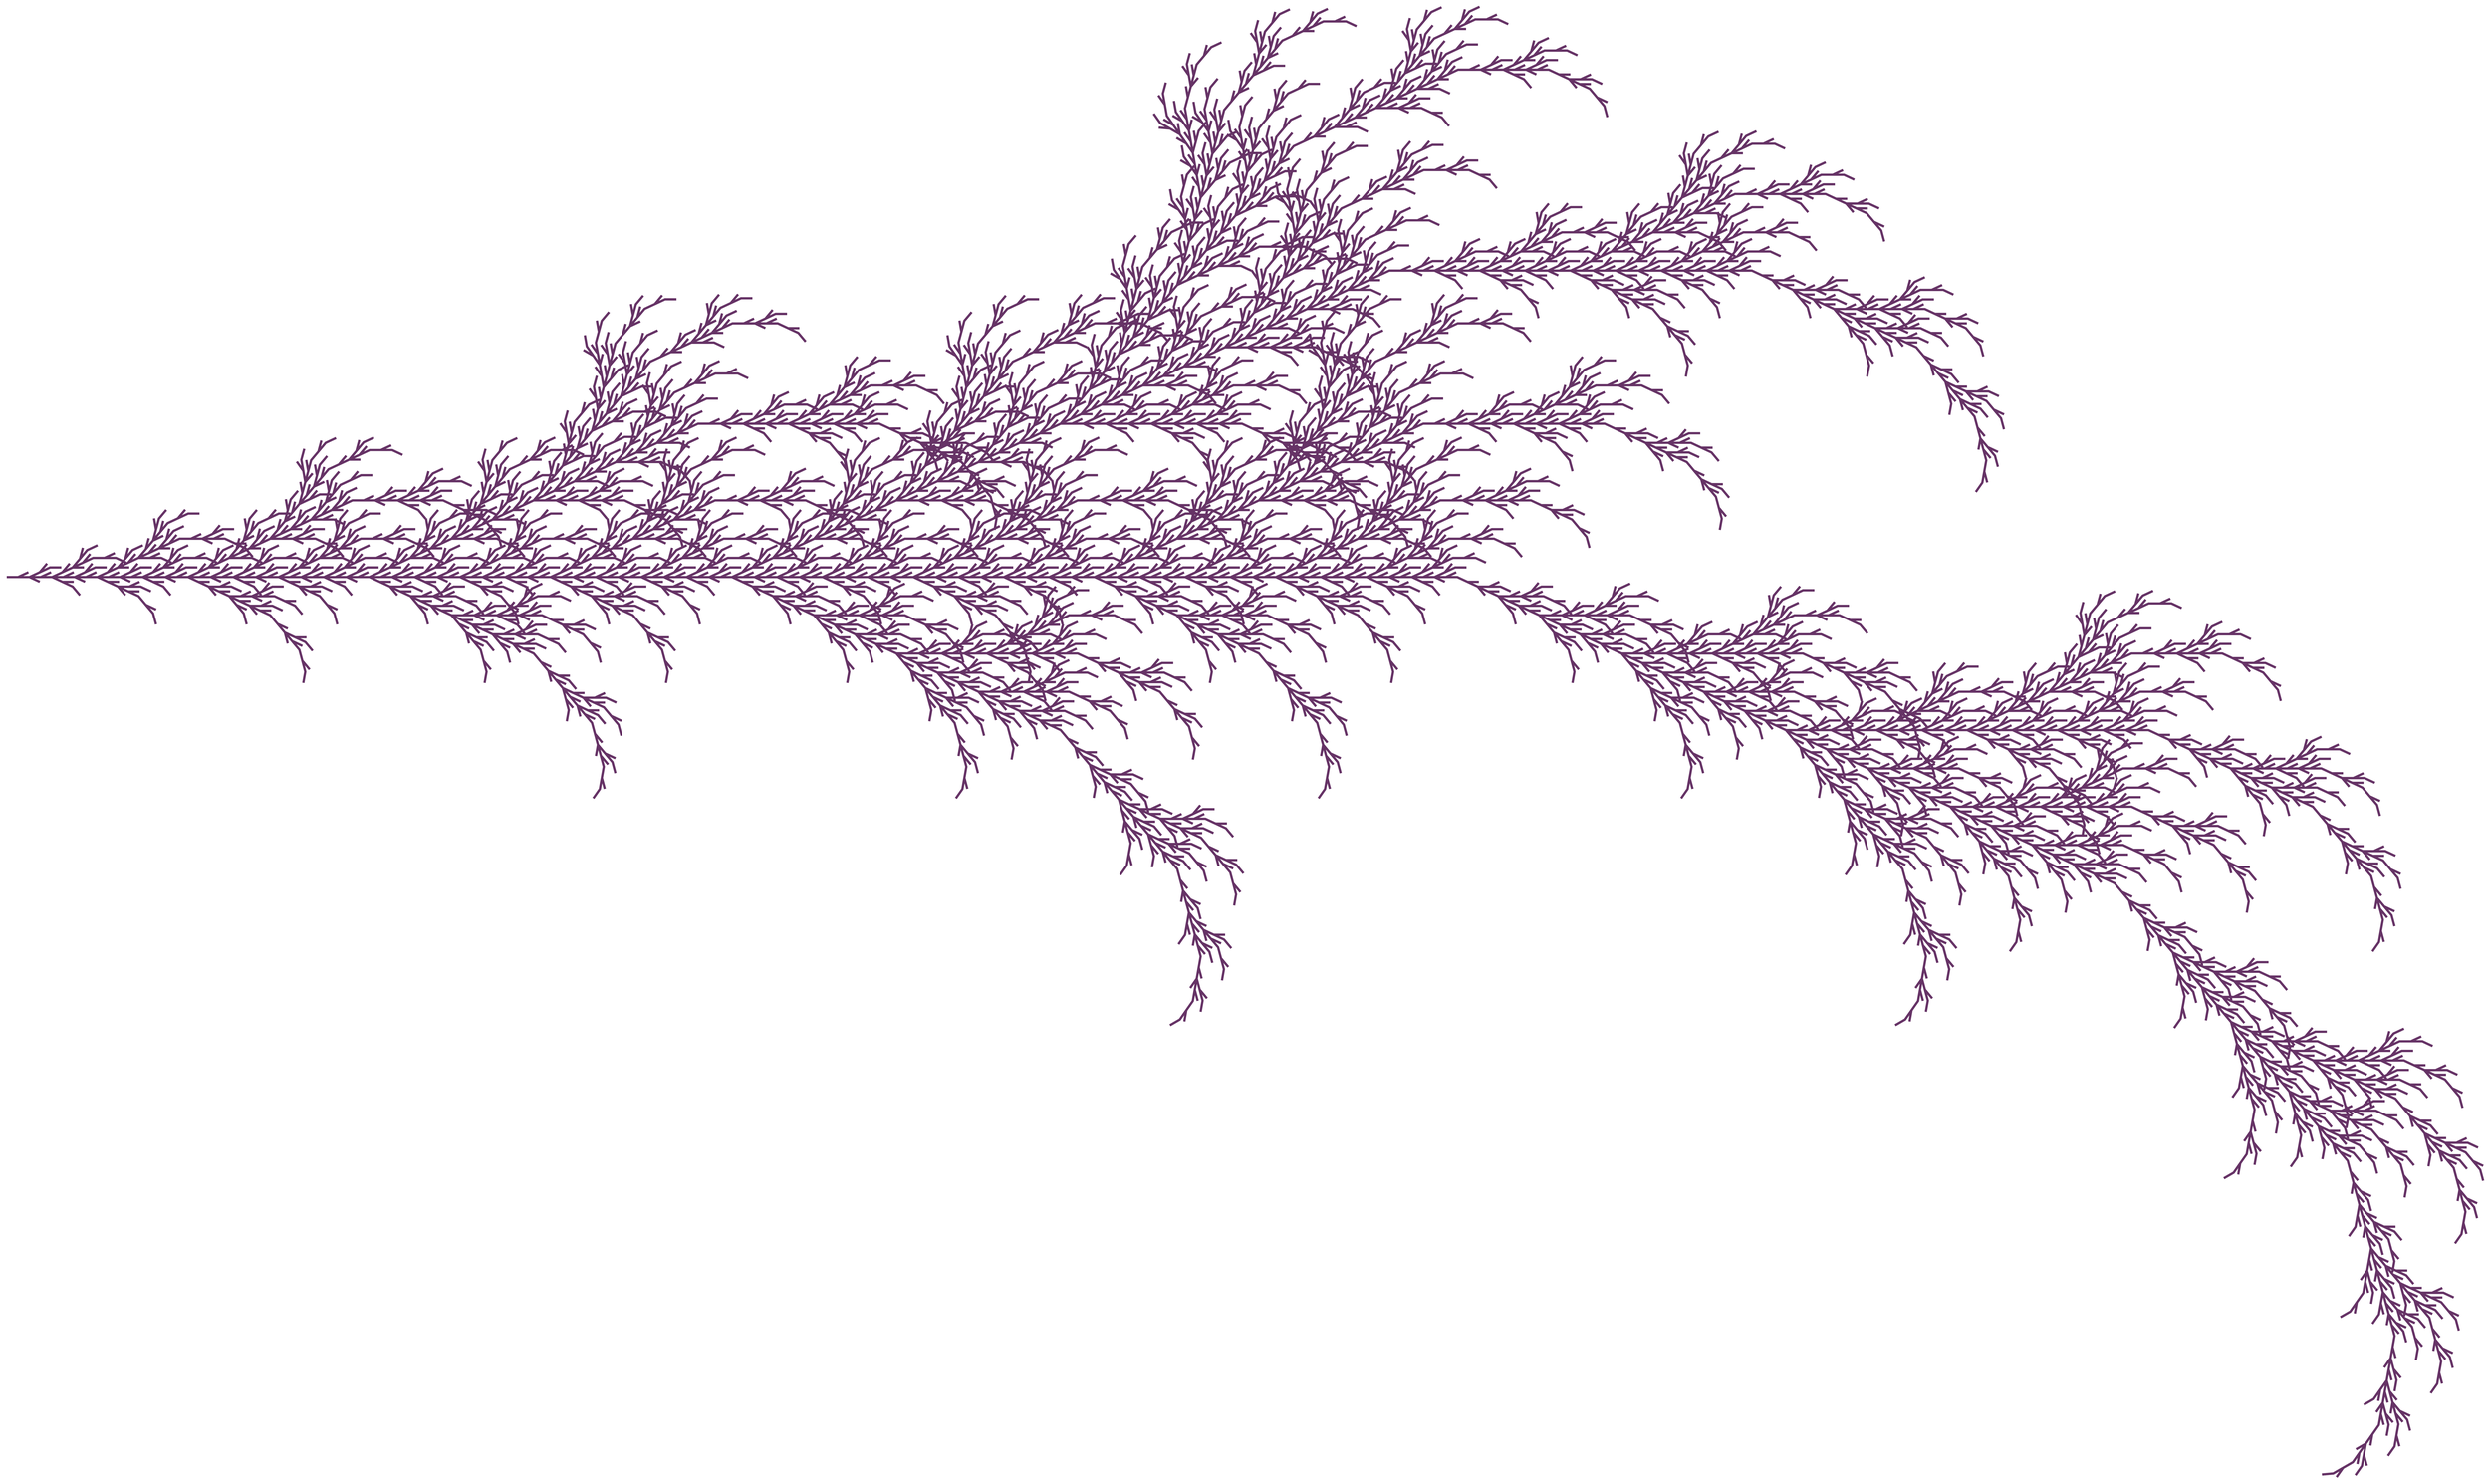
\begin{tikzpicture}
      \draw [pGreen,line width=4pt]
[l-system={fractal plant, step=20, angle=25, axiom=F, order=7}]
lindenmayer system;
\end{tikzpicture}
\end{document}